\documentclass[10pt]{article}

\usepackage[letterpaper,margin=0.72in]{geometry}
\usepackage{amsmath}
\usepackage{graphicx}
\usepackage{microtype}

\setlength{\parindent}{0pt}
\setlength{\parskip}{0.45em}
\graphicspath{{../../output/pdf/}}

\begin{document}

\section{Correctness-adjusted circuit cost}
\label{sec:correctness-adjusted-cost}

To estimate whether test-set hunting concealed rare failures, we evaluated 42
historical accepted circuits on a common corpus of exactly 50,000 valid
\texttt{secp256k1} point-addition input pairs. The sampled history contains
accepted submissions 1, 11, 21, and so on, together with submissions 401 and
405, the last accepted commit in the repository. The pairs were generated
pseudorandomly from the fixed seed
\texttt{ecdsafail-qxt-history-v1}, independently of each circuit's operation
stream. Every commit therefore received the same inputs. This paired design
makes the comparison reproducible and prevents any circuit from benefiting
from a specially hunted Fiat--Shamir test set.

\begin{figure}[htbp]
  \centering
  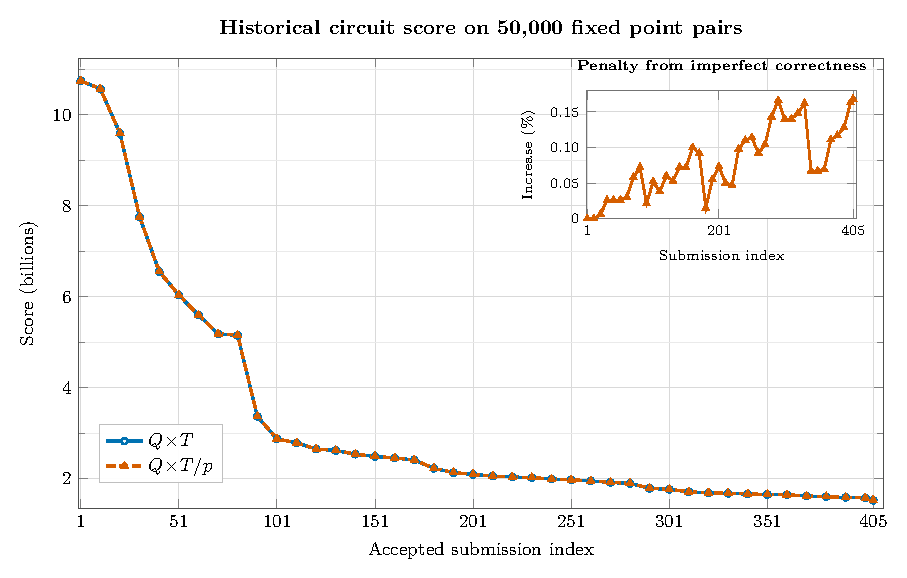
\includegraphics[width=0.98\linewidth]{qxt-history-plot.pdf}
  \caption{Raw and correctness-adjusted circuit scores across the sampled
  accepted submissions. The main panel plots $Q\!\times\!T$ and
  $Q\!\times\!T/p$; lower values are better. Because the two series are close
  at the full score scale, the inset reports the relative increase
  $100(1/p-1)$ in percent.}
  \label{fig:qxt-correctness-history}
\end{figure}

For each circuit, $Q$ is the peak number of live qubits, $T$ is the average
executed Toffoli count on the shared corpus, and $p$ is the observed fraction
of inputs that produced the expected classical affine output. We report the raw
score and its reliability-adjusted counterpart as
\[
  S_{\mathrm{raw}} = Q T,
  \qquad
  S_{\mathrm{adjusted}} = \frac{Q T}{p}.
\]
The factor $1/p$ penalizes unreliable circuits and can be interpreted as the
expected number of independent attempts per successful result when failures
are detectable. Here, ``correct'' refers specifically to the classical output;
phase and ancilla-cleanliness diagnostics were recorded separately and were
not folded into $p$.

Across the sampled commits, correctness ranged from $100\%$ to $99.832\%$, with
a median of $99.928\%$. Consequently, the adjustment was small: its maximum
relative increase was only $0.168\%$. For the final commit, the raw score was
$1.518693$ billion and the adjusted score was $1.521249$ billion. The raw and
adjusted curves therefore nearly overlap in Figure~\ref{fig:qxt-correctness-history},
although their separation is visible in the inset. No ranking reversal occurred
among the 42 sampled circuits: every circuit that ranked better under
$Q\!\times\!T$ also ranked better under $Q\!\times\!T/p$. This agreement is a
property of these measurements, not of the metric in general; a circuit with a
slightly lower raw score could rank worse after adjustment if its correctness
probability were sufficiently lower. From the first to the last sampled commit,
the raw score improved by a factor of $7.08$, while the adjusted score improved
by a factor of $7.07$.

\end{document}
